\bartchapterimage{halo}
\chapter{Halo mass functions}
\bartthumb{thumb_halo}
\minitoc%

\section{Theory}

\subsection{Definition}

By definition, the halo mass function by unit of comoving volume is the
number of halos with mass $M$ between $M$ and $M+\dd{M}$. If $N$ is
the number of halos, the halo mass function $\phi\left(M\right)$ can be
written:
%
\begin{equation}
    \phi\left(M\right)=\cfrac{\dd N^2}{\dd M\dd V}=\cfrac{\dd n}{\dd M}
\end{equation}
%
In this case, $n$ can be the comoving density of halos, or the cumulative
distribution function of the density. In the latter case, we have:
%
\begin{equation}
    n\left(M,z\right)=\int_0^M\phi\left(M,z\right)\dd M
\end{equation}
%
and so:
%
\begin{equation}
    \cfrac{\dd n}{\dd M}=\cfrac{\dd}{\dd M}\int_0^M\phi\left(M,z\right)\dd M=
    \cfrac{\dd}{\dd M}\left(\Phi\left(M,z\right)-\Phi\left(0,z\right)\right)=
    \phi\left(M,z\right)
\end{equation}
%
where $\Phi$ is a primitive of $\phi$.

\subsection{In practice}

\citet{Jenkins+01} found a general way to fit halo mass functions from
different cosmological simulations done with different cosmologies, allowing an
easy comparison between the different results. The halo mass function is
related to the variance of linear perturbations $\sigma$. A function
$f\left(\sigma\right)$ has been introduced for that, which is the fraction of
matter that is inside a halo of mass $M$ by units of $\ln\sigma^{-1}$. So:
%
\begin{equation}
    f\left(\sigma\right)=
        \cfrac{\dd\rho/\rho_m\left(z\right)}{\dd\ln\sigma^{-1}}=
        \cfrac{M}{\rho_m\left(z\right)}\frac{\dd n}{\dd\ln\sigma^{-1}}
\end{equation}
%
and the halo mass function is:
%
\begin{equation}
    \phi\left(M,z\right)=\cfrac{\dd\ln\sigma^{-1}}{\dd M}
    \cfrac{\rho_m\left({z}\right)}{M}f\left(\sigma\right)=
    \cfrac{\rho_m\left(z\right)}{M^2}\left|M\cfrac{\dd\ln\sigma}{\dd M}\right|
    f\left(\sigma\right)
\end{equation}
%
where the computation of $\sigma$ involves the power spectrum $P\left(k\right)$
and the Fourier space representation of the real space top hat filter
$\tilde{W}\left(k\right)$:
%
\begin{equation}
    \sigma^2\left(M\right) =
    \cfrac{1}{2\pi^2}\int_0^\infty P\left(k\right)
    \tilde{W}^2\left(k R\right) k^2\dd k
\end{equation}
%
and its logarithmic derivative is:
%
\begin{equation}
    \cfrac{\dd \ln\sigma}{\dd\ln M} = \cfrac{R}{12\pi^2\sigma^2}
    \int_0^\infty \cfrac{\dd W^2 \left(kR\right)}{\dd \left(kR\right)} k^3
    P \left(k\right) \dd k
\end{equation}
%
By definition, if we assume that all the matter is contained in dark matter
halos, summing over all the possible variance gives us the total mass, so:
%
\begin{equation}
    \int_{-\infty}^\infty f\left(\sigma\right)\dd\ln\sigma^{-1}=1
\end{equation}
%
The variance follows the evolution of the linear perturbations and must
growth with them, so we need to multiply it by the growth rate to extend the
expression to other redshifts.

\subsection{Window function}
\label{sub:window_function}

By definition, $\sigma$ is the variance of mass within a sphere of radius
$R$ containing mass $M$ with the mean density of the Universe. For this a
top-hat filter is used in real space corresponding to the sphere of radius
$R$. Its expression in the Fourier space is:
%
\begin{equation}
    W \left(kR\right) =
    \cfrac{3\left[\sin\left(kR\right) - kR \cos \left(kR\right)\right]}
    {{\left(kR\right)}^3}
\end{equation}
%
and we can explicitly write the derivative:
%
\begin{equation}
    \cfrac{\dd W^2 \left(x\right)}{\dd x} = \left[\sin x - x\cos x\right]
    \times \left[\sin x \left(1 - \cfrac{3}{x^3}\right) + 3\cfrac{\cos
    x}{x}\right]
\end{equation}

\subsection{Power spectrum}
\label{sub:power_spectrum}

In the context of the small perturbations theory, over-densities, expressed
as $\delta \left(\textbf{x}\right) = \left(\rho \left(\textbf{x}\right) -
\overline\rho\right) / \overline\rho$ growth linearly if they are small
(i.e.\ $\delta\ll1$). The power spectrum is the second moment of the
probability distribution function of the density perturbation field
expressed in the Fourier space:
%
\begin{equation}
    P \left(k\right) \propto
    \left\langle{\left|\delta_\textbf{k}\right|}^2\right\rangle
\end{equation}
%
Inflation models predicts a power spectrum of the form:
%
\begin{equation}
    P \left(k\right) \propto k^n
\end{equation}
%
where $n$ is the spectral index, close to 1. The different kind of matter
contribute to the power spectrum and in general diverge from this simple
model. The transfer function $T \left(k\right)$ accounts for this, as a
correction for the inflation model:
%
\begin{equation}
    P \left(k\right) \propto k^n T^2 \left(k\right)
\end{equation}
%
The transfer function is sensible to the model of dark matter matter and the
density of baryons through $\Omega_b$. The transfer function is very difficult
to compute precisely and thus we depend on the CAMB program \citep{Lewis+00}.

The power spectrum has a normalization not predictable by the theory, and must
be set by confrontation to the observations. For this, the variance of the
density field of the fluctuations within the smoothing window function of
radius $R=8 h^{-1}\mathrm{Mpc}$ is used, and by comparison with the value
obtained from observations with the galaxy distribution or other method, the
power spectrum is fully determined.

If we want to compute the power spectrum at different epochs, we must apply
the growth factor to the power spectrum, under the assumptions that
fluctuations evolution is linear. In this case $\delta \left(\textbf{x},
a\right) = D \left(a\right) \delta_i \left(\textbf{x}\right)$, where
$D\left(a\right)$ is the growth factor and $a$ the scale factor. For the
growing mode of perturbations:
%
\begin{equation}
    D \left(z\right) = \cfrac{5\Omega_m}{2}E \left(z\right)
    \int_z^\infty \cfrac{\left(1+z'\right)}{E^3\left(z'\right)} \dd z'
\end{equation}
%
with:
%
\begin{equation}
    E \left(z\right) = \cfrac{H \left(z\right)}{H_0} =
    \sqrt{\Omega_m {\left(1+z\right)}^3 + \Omega_\Lambda}
\end{equation}
%
for a flat Universe (see \citet{Hogg+99, Carroll+92}). The growth factor to
apply to power spectrum is:
%
\begin{equation}
    d \left(z\right) = \cfrac{D \left(z\right)}{D \left(z=0\right)}
\end{equation}

The power spectrum and the variance of the perturbations evolve in the
following way:
%
\begin{align}
    P \left(k, z\right) &= d^2 \left(z\right) P \left(k, 0\right)
    \nonumber\\
    \sigma \left(M, z\right) &= d \left(z\right) \sigma \left(M,0\right)
    \nonumber\\
\end{align}

\section{In practice}
\label{sec:in_practice}

\subsection{Approximation}
\label{sub:approximation}

As described above, the computation of the density fluctuation variance
implies to compute a integral that must be done numerically since the power
spectrum doesn't have an analytical form. Hence, the halo mass function
computation needs to do two integrals numerically, which is time consuming.
Hopefully, in~\cite{vandenBosch+02}, there is a good approximation for the
variance of the density field:
%
\begin{equation}
    \sigma\left(M\right)=\sigma_8\frac{f\left(u\right)}{f\left(u_8\right)}
\end{equation}
%
with the function $f$:
%
\begin{equation}
    f\left(u\right)=
    64.087 {\left(1 + 1.074 u^{0.3} - 1,581 u^{0.4} +
        0.954 u^{0.5} - 0.185 u^{0.6}\right)}^{-10}
\end{equation}
%
and $u$, $u_8$ which are:
%
\begin{eqnarray}
    u & = & 3.804 10^{-4}\Gamma{\left(\frac{Mh}{\Omega_{m,0}}\right)}^{1/3}
        \nonumber\\
    u_8 & = & 32\Gamma\nonumber\\
    \Gamma & = &
        \Omega_{m,0}h\exp
        \left[-\Omega_b\left(1+\sqrt{2h}/\Omega_{m,0}\right)\right]\nonumber\\
\end{eqnarray}
%
Now, with this approximation, we can compute the derivative of
$\sigma$ and:
%
\begin{equation}
    {\left(M\frac{\dd\ln\sigma}{\dd M}\right)}^{-1}+\undemi =
    \frac{\left(-0.000310111 X^{1.7} + 0.00225895 X^{1.6} -
        0.00505879 X^{1.5} - 0.1 X^{1.2}\right)}
        {\left(-0.000328357 X^{1.8} + 0.00310111 X^{1.7} -
        0.0090358 X^{1.6} + 0.0101176 X^{1.5}\right)}
\end{equation}
%
with:
%
\begin{equation}
    X=\Gamma
    \sqrt[3]{\frac{h M}{\Omega _{m,0}}}
\end{equation}
%

In \bartreffigure{sigma}, we show the comparison between the variance
computed with the transfer function obtained from the CAMB program and the
approximation of \citet{vandenBosch+02}.
%
\begin{figure}[htb]
    \centering
    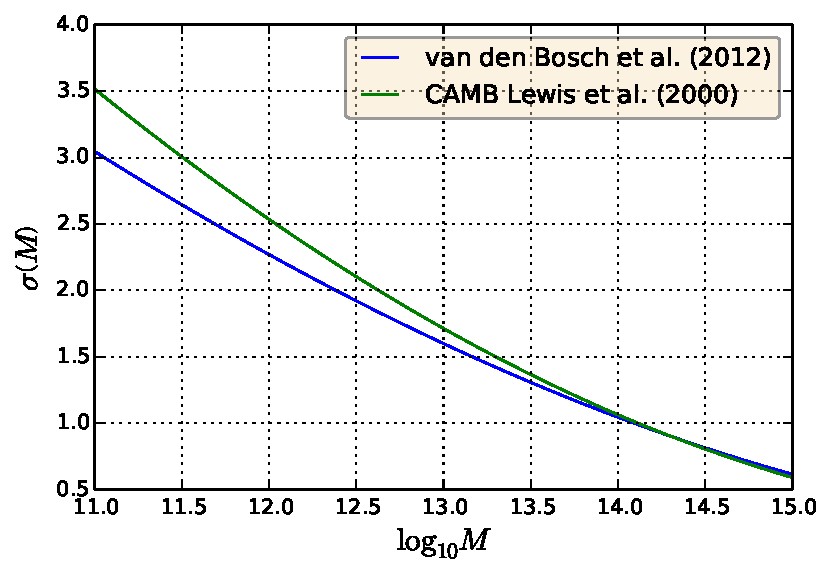
\includegraphics[width=0.6\linewidth]{figures/hmf/sigma.pdf}
    \caption{Comparison between the variance of the density fluctuation
        computed numerically from the transfer function obtained from CAMB
        \citep{Lewis+00} in \emph{green} and the approximation from
        \citet{vandenBosch+02} in \emph{blue}. Models diverge at low masses
        but the computation of the halo mass function seems to not be
    affected by this divergences.\label{fig:sigma}}
\end{figure}
%
The approximation diverges from the theoretical computation involving the
transfer function, but when used for the computation of the halo mass
function, discrepancies are not significant.

\subsection{Halo mass function models}
\label{sub:halo_mass_function_models}

We put here a list of some common models for the halo mass function, and
used in the thesis for various comparisons. A detailed list can be found in
\citet{Murray+13}.

\begin{table}
    \centering
    \caption{A table of some models for the halo mass
    function.\label{tab:hmf}}
    \begin{tabular}{cp{6.5cm}p{5cm}}
        \toprule
        Model & $f \left(\sigma\right)$ & Parameters\\
        \midrule
        \citet{Warren+06} &
        $f\left(\sigma\right)=
        A\left(\sigma^{-a}+b\right)\exp\left(-\cfrac{c}{\sigma^2}\right)$ &
        $A=0.7234$, \newline
        $a=1.625$, \newline
        $b=0.2538$, \newline
        $c=1.1982$
        \\
        \citet{Courtin+11} &
        $f\left(\sigma\right)=
        A{\left(\frac{2a}{\pi}\right)}^\undemi
        \frac{\delta_c}{\sigma}\left(1+
        {\left(\frac{\sqrt{a}\delta_c}{\sigma}\right)}^{-2p}\right)$\newline
        $\times\exp\left(-\frac{\delta_c^2{a}}{2\sigma^2}\right)$ &
        $A=0.348$, \newline
        $a=0.695$, \newline
        $p=0.1$, \newline
        $\delta_c=1.673$ \\
        \citet{Crocce+10} &
        $f\left(\sigma\right)=
        A\left(\sigma^{-a}+b\right)\exp\left(-\cfrac{c}{\sigma^2}\right)$ &
        $A\left(z\right)=0.58{\left(1+z\right)}^{-0.13}$,\newline
        $a\left(z\right)=1.37{\left(1+z\right)}^{-0.15}$,\newline
        $b\left(z\right)=0.3{\left(1+z\right)}^{-0.084}$,\newline
        $c\left(z\right)=1.036{\left(1+z\right)}^{-0.024}$
        \\
        \citet{Jenkins+01} &
        $f\left(\sigma\right)=
        A\exp\left(-\left|\ln\sigma^{-1}+a\right|^b\right)$ &
        $A=0.315$, \newline
        $a=0.61$, \newline
        $b=3.8$ \\
        \citet{Tinker+08} &
        $f\left(\sigma\right)=
        A\left({\left(\frac{\sigma}{b}\right)}^{-a}+1\right)
        \exp\left(-\cfrac{c}{\sigma^2}\right)$ &
        $A\left(z\right)=A_0{\left(1+z\right)}^{-0.14}$,\newline
        $a\left(z\right)=a_0{\left(1+z\right)}^{-0.06}$,\newline
        $b\left(z\right)=b_0{\left(1+z\right)}^{-\alpha}$,\newline
        $\log_{10}\alpha=
        -{\left[\cfrac{0.75}{\ln\left(\Delta/75\right)}\right]}^{1.2}$,\newline
        $A_0=0.1\log_{10}\Delta-0.05$,\newline
        $a_0=1.43+{\left(\log_{10}\Delta-2.3\right)}^{1.5}$,\newline
        $b_0=1.0+{\left(\log_{10}\Delta-1.6\right)}^{-1.5}$,\newline
        $c_0=1.2+{\left(\log_{10}\Delta-2.35\right)}^{1.6}$ \\
        \bottomrule
    \end{tabular}
\end{table}
